\documentclass{article}

\usepackage{amsmath,amssymb}
\usepackage{tikz}
\usepackage{pgfplots}
\usepackage{xcolor}
\usepackage[left=2.1cm,right=3.1cm,bottom=3cm,footskip=0.75cm,headsep=0.5cm]{geometry}
\usepackage{enumerate}
\usepackage{enumitem}
\usepackage{marvosym}
\usepackage{tabularx}
\usepackage[amsmath,thmmarks,standard]{ntheorem}
\usepackage{mathtools}

\usepackage[utf8]{inputenc}

\renewcommand*{\arraystretch}{1.4}
\newcommand{\E}{\mathbb{E}}

\newcolumntype{L}[1]{>{\raggedright\arraybackslash}p{#1}}
\newcolumntype{R}[1]{>{\raggedleft\arraybackslash}p{#1}}
\newcolumntype{C}[1]{>{\centering\let\newline\\\arraybackslash\hspace{0pt}}m{#1}}

\DeclareMathOperator{\tr}{tr}
\DeclareMathOperator{\Var}{Var}
\DeclareMathOperator{\Cov}{Cov}
\renewcommand{\E}{\mathbb{E}}

\newtheorem{thm}{Theorem}
\newtheorem{lem}{Lemma}

\title{\textbf{Einführung in die Produktion, Tutorium 3}}
\author{\textsc{Henry Haustein}}
\date{}

\begin{document}
	\maketitle
	
	\section*{Aufgabe 7}
	\begin{enumerate}[label=(\alph*)]
		\item Zielfunktion $G = (7-5)x_B + (3.5-2.3)x_K + (2.3-2.4)x_L + (3.2-3.5)x_T \to \max$. Man sieht sehr gut, dass es sich nicht lohnt die Produkte $x_L$ und $x_T$ zu produzieren, da sie mehr kosten als sie einbringen. Es gilt also $x_L=x_T=0$. Die Nebenbedingen dazu lauten dann
		\begin{align}
			6x_B + 3x_K &\le 3900 \notag \\
			2x_B + 2.5x_K &\le 3900 \notag \\
			2.5x_B + 3x_K &\le 3900 \notag \\
			x_B &\le 600 \notag \\
			x_K &\le 200 \notag \\
			x_B,x_K &\ge 0 \notag
		\end{align}
		Unter Nutzung von https://www2.wiwi.uni-jena.de/Entscheidung/tenor/ ergibt sich eine Lösung von
		\begin{center}
			\begin{tabular}{c|cc}
				& \textbf{Ergebnis} & \textbf{Opp-Kosten} \\
				\hline
				$x_B$ & 550 & 0 \\
				$x_K$ & 200 & 0 \\
				$y_1$ & 0 & $\frac{1}{3}$ \\
				$y_2$ & 1925 & 0 \\
				$y_3$ & 2300 & 0 \\
				$y_4$ & 50 & 0 \\
				$y_5$ & 0 & $\frac{1}{5}$ \\
				$F$ & 1340 & \\
			\end{tabular}
		\end{center}
		Es sollten also 550 Einheiten Baldrianwurzel und 200 Einheiten Kamillenblüten hergestellt werden. Das liefert einen Deckungsbeitrag von 1340 GE.
		\item Graphische Lösung:
		\begin{center}
			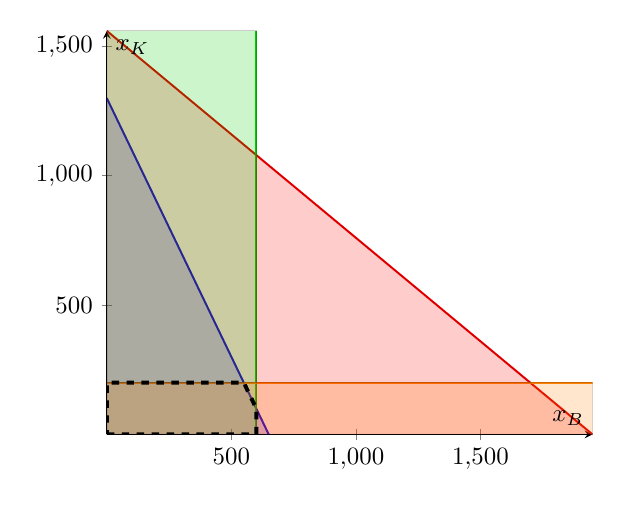
\begin{tikzpicture}[scale=0.9]
			\begin{axis}[
			xmin=0, xmax=1950, xlabel=$x_B$,
			ymin=0, ymax=1560, ylabel=$x_K$,
			samples=400,
			axis x line=middle,
			axis y line=middle,
			domain=0:1950,
			]
			\draw[blue,thick] (axis cs: 0,1300) -- (axis cs: 650,0);
			\draw[red,thick] (axis cs: 0,1560) -- (axis cs: 1950,0);
			\draw[green!80!black,thick] (axis cs: 600,0) -- (axis cs: 600,1560);
			\draw[orange,thick] (axis cs: 0,200) -- (axis cs: 1950,200);
			
			\draw[fill=blue,opacity=0.2] (axis cs: 0,0) -- (axis cs: 0,1300) -- (axis cs: 650,0) -- (axis cs: 0,0);
			\draw[fill=red,opacity=0.2] (axis cs: 0,0) -- (axis cs: 0,1560) -- (axis cs: 1950,0) -- (axis cs: 0,0);
			\draw[fill=green!80!black,opacity=0.2] (axis cs: 0,0) rectangle (axis cs: 600,1560);
			\draw[fill=orange,opacity=0.2] (axis cs: 0,0) rectangle (axis cs: 1950,200);
			
			\draw[ultra thick,dashed] (axis cs: 0,0) -- (axis cs: 600,0) -- (axis cs: 600,100) -- (axis cs: 550,200) -- (axis cs: 0,200) -- (axis cs: 0,0);
			
			\end{axis}
			\end{tikzpicture}
			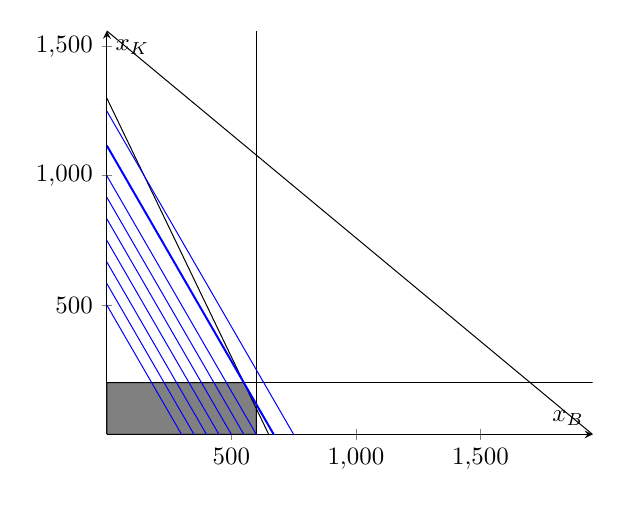
\begin{tikzpicture}[scale=0.9]
			\begin{axis}[
			xmin=0, xmax=1950, xlabel=$x_B$,
			ymin=0, ymax=1560, ylabel=$x_K$,
			samples=400,
			axis x line=middle,
			axis y line=middle,
			domain=0:1950,
			]
			\draw (axis cs: 0,1300) -- (axis cs: 650,0);
			\draw (axis cs: 0,1560) -- (axis cs: 1950,0);
			\draw (axis cs: 600,0) -- (axis cs: 600,1560);
			\draw (axis cs: 0,200) -- (axis cs: 1950,200);
			
			\draw[fill=gray] (axis cs: 0,0) -- (axis cs: 600,0) -- (axis cs: 600,100) -- (axis cs: 550,200) -- (axis cs: 0,200) -- (axis cs: 0,0);
			
			\addplot[smooth,mark=none,blue] {(600-2*x)/1.2};
			\addplot[smooth,mark=none,blue] {(700-2*x)/1.2};
			\addplot[smooth,mark=none,blue] {(800-2*x)/1.2};
			\addplot[smooth,mark=none,blue] {(900-2*x)/1.2};
			\addplot[smooth,mark=none,blue] {(1000-2*x)/1.2};
			\addplot[smooth,mark=none,blue] {(1100-2*x)/1.2};
			\addplot[smooth,mark=none,blue] {(1200-2*x)/1.2};
			\addplot[smooth,mark=none,blue,thick] {(1340-2*x)/1.2};
			\addplot[smooth,mark=none,blue] {(1500-2*x)/1.2};
			
			
			\end{axis}
			\end{tikzpicture}
		\end{center}
		Das optimale Produktionsprogramm stellt 550 $x_B$ und 200 $x_K$ her. Das liefert einen Gewinn von 1340.
	\end{enumerate}

	\section*{Aufgabe 8}
	\begin{enumerate}[label=(\alph*)]
		\item Es gilt DB = Erlös - variable Kosten. Es gilt also für $P_1$:
		\begin{align}
			DB_{P_1} &= 259 - \underbrace{(1\cdot 120)}_{\text{Blech}} - \underbrace{(1.5\cdot 6)}_{\text{Farbe}} - \underbrace{(3\cdot 30)}_{\text{Arbeit}} \notag \\
			&= 259-120-9-90 \notag \\
			&= 40 \notag
		\end{align}
		Und für $P_2$:
		\begin{align}
			DB_{P_2} &= 317 - \underbrace{(1.5\cdot 120)}_{\text{Blech}} - \underbrace{(2\cdot 6)}_{\text{Farbe}} - \underbrace{(2.5\cdot 30)}_{\text{Arbeit}} \notag \\
			&= 317-180-12-75 \notag \\
			&= 50 \notag
		\end{align}
		\item Zielfunktion: $G=40x_1 + 50x_2 \to\max$ unter den Nebenbedingungen
		\begin{align}
			1x_1 + 1.5x_2 &\le 750 \notag \\
			1.5x_1 + 2x_2 &\le 1200 \notag \\
			3x_1 + 2.5x_2 &\le 2000 \notag \\
			x_2 &\le 80 \notag \\
			x_1,x_2 &\ge 0 \notag
		\end{align}
		\item Graphische Lösung
		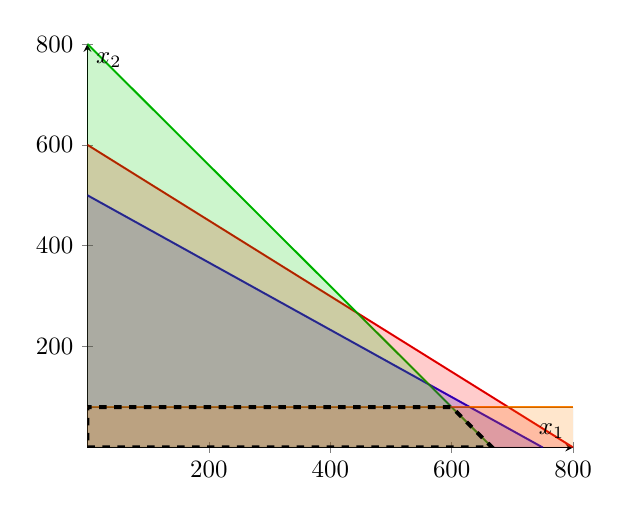
\begin{tikzpicture}[scale=0.9]
		\begin{axis}[
		xmin=0, xmax=800, xlabel=$x_1$,
		ymin=0, ymax=800, ylabel=$x_2$,
		samples=400,
		axis x line=middle,
		axis y line=middle,
		domain=0:800,
		]
		\draw[blue,thick] (axis cs: 0,500) -- (axis cs: 750,0);
		\draw[red,thick] (axis cs: 0,600) -- (axis cs: 800,0);
		\draw[green!80!black,thick] (axis cs: 666.67,0) -- (axis cs: 0,800);
		\draw[orange,thick] (axis cs: 0,80) -- (axis cs: 800,80);
		
		\draw[fill=blue,opacity=0.2] (axis cs: 0,0) -- (axis cs: 0,500) -- (axis cs: 750,0) -- (axis cs: 0,0);
		\draw[fill=red,opacity=0.2] (axis cs: 0,0) -- (axis cs: 0,600) -- (axis cs: 800,0) -- (axis cs: 0,0);
		\draw[fill=green!80!black,opacity=0.2] (axis cs: 0,0) -- (axis cs: 666.67,0) -- (axis cs: 0,800) -- (axis cs: 0,0);
		\draw[fill=orange,opacity=0.2] (axis cs: 0,0) rectangle (axis cs: 800,80);
		
		\draw[ultra thick,dashed] (axis cs: 0,0) -- (axis cs: 666.67,0) -- (axis cs: 600,80) -- (axis cs: 0,80) -- (axis cs: 0,0);
		
		\end{axis}
		\end{tikzpicture}
		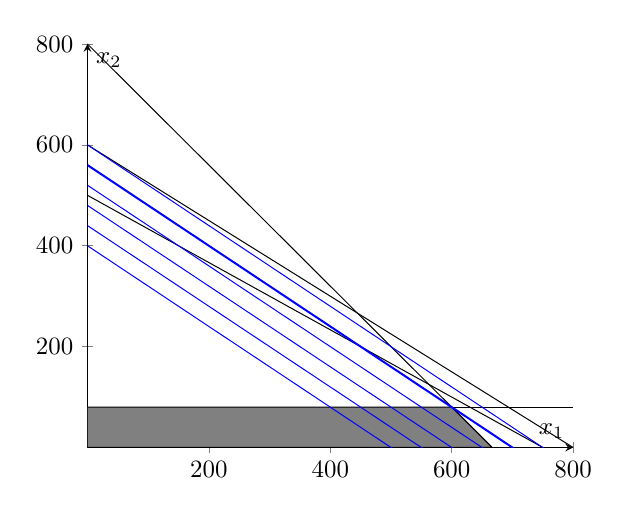
\begin{tikzpicture}[scale=0.9]
		\begin{axis}[
		xmin=0, xmax=800, xlabel=$x_1$,
		ymin=0, ymax=800, ylabel=$x_2$,
		samples=400,
		axis x line=middle,
		axis y line=middle,
		domain=0:800,
		]
		\draw (axis cs: 0,500) -- (axis cs: 750,0);
		\draw (axis cs: 0,600) -- (axis cs: 800,0);
		\draw (axis cs: 666.67,0) -- (axis cs: 0,800);
		\draw (axis cs: 0,80) -- (axis cs: 800,80);
		
		\draw[fill=gray] (axis cs: 0,0) -- (axis cs: 666.67,0) -- (axis cs: 600,80) -- (axis cs: 0,80) -- (axis cs: 0,0);
		
		\addplot[smooth,mark=none,blue] {(20000-40*x)/50};
		\addplot[smooth,mark=none,blue] {(22000-40*x)/50};
		\addplot[smooth,mark=none,blue] {(24000-40*x)/50};
		\addplot[smooth,mark=none,blue] {(26000-40*x)/50};
		\addplot[smooth,mark=none,blue,thick] {(28000-40*x)/50};
		\addplot[smooth,mark=none,blue] {(30000-40*x)/50};
		\end{axis}
		\end{tikzpicture}
		Liefert ein optimales Produktionsprogramm von 600 $x_1$ und 80 $x_2$. Das ergibt einen Gewinn von 28000.
		\item Es werden nur die Absatzbeschränkung und die Beschränkung der Arbeitszeit vollständig in Anspruch genommen.
	\end{enumerate}

	\section*{Aufgabe 9}
		\begin{enumerate}[label=(\alph*)]
		\item Zielfunktion: $G=20x_1 + 30x_2 + 25x_3 \to\max$ unter den Nebenbedingungen
		\begin{align}
			2x_1 + 1x_2 + 2x_3 &\le 60 \notag \\
			2x_1 + 4x_2 + x_3 &\le 100 \notag
		\end{align}
		\item Man sieht, dass - analog zur Spalte $x_3$, für $A=0$ gelten muss. Für die anderen Variablen gilt:
		\begin{align}
			-\frac{1}{7}\cdot 25 + B\cdot 30 &= 5 \notag \\
			\frac{4}{7}\cdot 25 - \frac{1}{7}\cdot 30 &= C \notag \\
			20\cdot 25 + 20\cdot 30 &= D \notag
		\end{align}
		ergibt $B=\frac{2}{7}$, $C=10$ und $D=1100$.
		\item Die Schlupfvariable für die Fertigung ist $y_2$, das heißt eine Zeiteinheit mehr bei der Fertigung ergibt 5 GE mehr Deckungsbeitrag.
		\item Wird $x_1$ produziert, findet eine Verdrängung von $\frac{2}{7}x_2$ und $\frac{6}{7}x_3$ statt. Der Deckungsbeitrag sinkt um 10 GE\footnote{Statt dies aus dem Tableau auszulesen, kann man es auch einfach berechnen: Wird eine Einheit $x_1$ produziert, steigt der DB um 20, aber durch die Verdrängung von $x_2$ und $x_3$ sinkt der DB um $\frac{2}{7}\cdot 30 + \frac{6}{7}\cdot 25=30$}. 
	\end{enumerate}
	
\end{document}